\documentclass[aspectratio=169, handout]{beamer}
\usepackage[utf8]{inputenc}
\usepackage{amsmath}
\usepackage{tikz}
\usepackage{dsfont}
\usepackage{opensans}

\usetikzlibrary{math} 
\usetikzlibrary{decorations.pathmorphing}

\usetheme{NOVASBE}

\title[]{4509 - Bridging Mathematics}
\subtitle{Correspondences}
\author[P. Fagandini]{Paulo Fagandini}
\institute{}
\date{}

\newtheorem{defenition}{Definition}[section]
\newtheorem{proposition}{Conjecture}[section]

\begin{document}

\begin{frame}
    \begin{definition}
        A \textbf{correspondence} or \textbf{set-valued function} is a function that maps elements from one set, the domain, to subsets of another set.
        \begin{align*}
            \Gamma:A&\twoheadrightarrow B\\
            a\in A&\rightarrow \Gamma(a)\subseteq B
        \end{align*}
    \end{definition}

    Any idea on how to turn $\Gamma$ into a function?

\end{frame}

\begin{frame}{Example}
    
    \tikzmath{\x1 = 0; \y1 = 1.5;
              \x2 = 3; \y2 = 2;
              \x3 = 2; \y3 = 0.5;
              \x4 = 4.5; \y4 = 1;
             } 
    \begin{figure}
        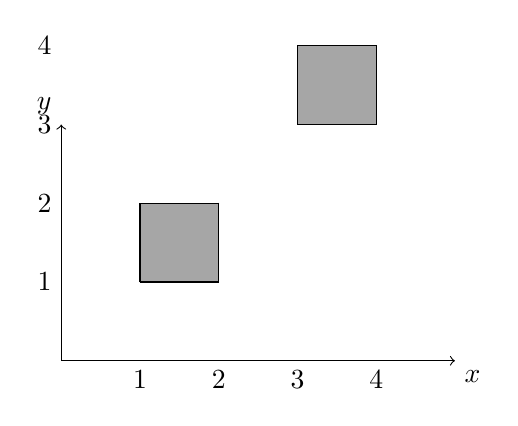
\begin{tikzpicture}

            \draw (\x1, \y1) -- (\x2,\y2);

            \draw[<->] (0,3) node[above left]{$y$} -- (0,0) --  (5,0)node[below right]{$x$};

            \draw[fill=gray!70] (\x1,\y1) -- (\x1, \y2) -- (\x2, \y2) -- (\x2, \y1) -- (\x1, \y1);
            \draw[fill=gray!70] (\x3,\y3) -- (\x3, \y4) -- (\x4, \y4) -- (\x4, \y3) -- (\x3, \y3);

            \foreach \val in {\x1, \x2, \x3, \x4}
            {
                \draw (\val,0) node[below] {$\val$};
            }

            \foreach \val in {\y1, \y2, \y3, \y4}
            {
                \draw (0,\val) node[left] {$\val$};
            }

         \end{tikzpicture}
    \end{figure}

    \[
        \Gamma(x) = 
            \begin{cases}
                [\y1, \y2] & \text{if } x \in [\x1, \x3] \\
                [\y1,\y2] \cup [\y3,\y4] & \text{if } x \in [\x3,\x2]\\ 
                [\y3, \y4] & \text{if } x \in [\x2, \x4]
            \end{cases}
    \]

\end{frame}

\begin{frame}{Example}

    The budget set is another often used example in economics. For a given $W$, we have:

    \[B(p) = \{x\in\mathds{R}^n | p'x\leq W\}\]

    Then $B(p)$ is a correspondence $B: \mathds{R}^n_{++}\twoheadrightarrow\mathds{R}^n_+$.
    
\end{frame}

\begin{frame}
    \begin{definition}
        Let $\Gamma:X\twoheadrightarrow Y$. A \textbf{selection} is a function $g:X\rightarrow Y$ such that $g(x)\in \Gamma(x)$ $\forall x\in X$.
    \end{definition}
\end{frame}

\begin{frame}
    \begin{definition}
        A correspondence $\Gamma$ is said to be \textbf{upper-hemicontinuous (uhc)} at $x_0\in X$ if, for any open set such that $V$ \[f(x_0)\subseteq V \Rightarrow \exists \text{ open } U\subseteq X:[x_0\in U \text{ and } x\in U\Rightarrow f(x)\subseteq V] \]
    \end{definition}

    \pause

    \begin{definition}
        A correspondence $\Gamma$ is said to be \textbf{uhc} if $\Gamma$ is uhc $\forall x\in X$.
    \end{definition}
\end{frame}

\begin{frame}
    \begin{definition}
        A correspondence $\Gamma$ is said to be \textbf{lower-hemicontinuous (lhc)} at $x\in X$ if for any open set $V$ such that
        \[f(x_0)\cap V \neq\emptyset\Rightarrow \exists \text{ open } U\subseteq X: [x_0\in U\text{ and }x\in U\Rightarrow f(x)\cap V\neq \emptyset]\]
        
    \end{definition}

    \begin{definition}
        A correspondence $\Gamma$ is said to be \textbf{lhc} if $\Gamma$ is lhc $\forall x\in X$.
    \end{definition}
\end{frame}

\begin{frame}{Example}

    Consider the correspondence $\Gamma$, defined as:

    \begin{align*}
        \Gamma(x)=
            \left\{
                \begin{array}{cl}
                    [1,2]&, 0\leq x \leq 3 \\
                    \left[\frac{1}{2},\frac{5}{2}\right] &, x\geq 3
                \end{array}
            \right.
    \end{align*}

    \begin{figure}
        
        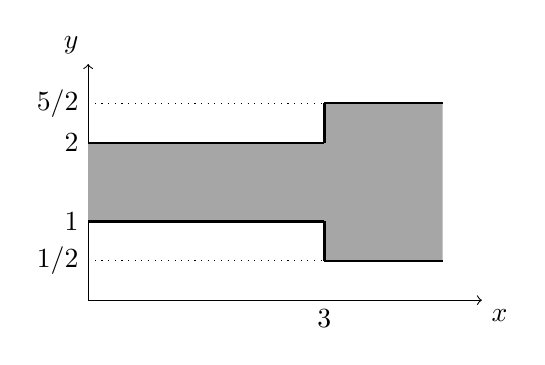
\begin{tikzpicture}
            \draw[<->] (0,3) node[above left]{$y$} -- (0,0) --  (5,0)node[below right]{$x$};

            \fill[gray!70] (0,1) -- (0,2) -- (3,2) -- (3,{5/2}) -- (4.5,{5/2}) -- (4.5,{1/2}) -- (3,{1/2}) -- (3,1) -- (0,1);

            \draw[thick] (0,2) -- (3,2);
            \draw[thick] (0,1) -- (3,1);

            \draw[thick] (3,2) -- (3,{5/2});
            \draw[thick] (3,1) -- (3,{1/2});

            \draw[thick] (3,{5/2}) -- (4.5,{5/2});
            \draw[thick] (3,{1/2}) -- (4.5,{1/2});

            \draw[dotted] (0, {5/2}) -- (3, {5/2});
            \draw[dotted] (0, {1/2}) -- (3, {1/2});

            \draw (3,0) node[below]{$3$};
            \draw (0,{1/2}) node[left]{$1/2$};
            \draw (0,1) node[left]{$1$};
            \draw (0,2) node[left]{$2$};
            \draw (0,{5/2}) node[left]{$5/2$};                      

         \end{tikzpicture}
    \end{figure}

\end{frame}

\begin{frame}{Example} 
        Consider the correspondence $\Gamma$, defined as:

    \begin{align*}
        \Gamma(x)=
            \left\{
                \begin{array}{cl}
                    [1,2]&, 0\leq x \leq 3 \\
                    \left[\frac{1}{2},\frac{5}{2}\right] &, x> 3
                \end{array}
            \right.
    \end{align*}

    \begin{figure}
        
        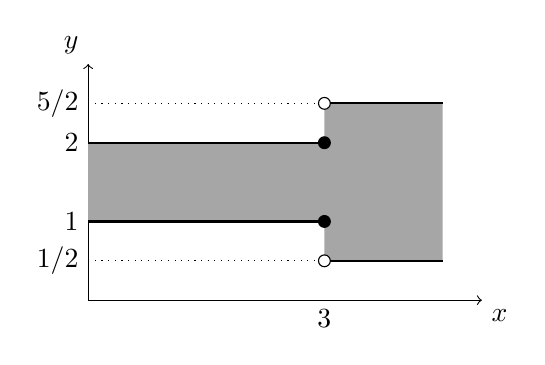
\begin{tikzpicture}
            \draw[<->] (0,3) node[above left]{$y$} -- (0,0) --  (5,0)node[below right]{$x$};

            \fill[gray!70] (0,1) -- (0,2) -- (3,2) -- (3,{5/2}) -- (4.5,{5/2}) -- (4.5,{1/2}) -- (3,{1/2}) -- (3,1) -- (0,1);

            \draw[thick] (0,2) -- (3,2);
            \draw[thick] (0,1) -- (3,1);

            \draw[thick] (3,{5/2}) -- (4.5,{5/2});
            \draw[thick] (3,{1/2}) -- (4.5,{1/2});

            \draw[dotted] (0, {5/2}) -- (3, {5/2});
            \draw[dotted] (0, {1/2}) -- (3, {1/2});

            \draw (3,0) node[below]{$3$};
            \draw (0,{1/2}) node[left]{$1/2$};
            \draw (0,1) node[left]{$1$};
            \draw (0,2) node[left]{$2$};
            \draw (0,{5/2}) node[left]{$5/2$};

            \draw [fill=white] (3,{1/2}) circle (0.075);
            \draw [fill=white] (3,{5/2}) circle (0.075);

            \draw [fill=black] (3,2) circle (0.075);
            \draw [fill=black] (3,1) circle (0.075);
                       

         \end{tikzpicture}
    \end{figure}
\end{frame}

\begin{frame}
    \begin{definition}
        A correspondence is said to be \textbf{continuous} if it is upper and lower hemicontinuous.
    \end{definition}
\end{frame}

\begin{frame}{The case of the Budget Set}
    Consider the correspondence $B: \mathds{R}^n_{++}\twoheadrightarrow\mathds{R}^n_+$:
    \[B(p) = \{x\in\mathds{R}^n_+ | p'x\leq p'x_0\}\]
    where $x_0\in \mathds{R}^n_{+}$ is the initial endowment of the consumer.
    
    \pause

    Trivially $x_0\in B(p)\ \forall p\in\mathds{R}^n_{++}$.

    \pause

    Well established is also, the fact that changing $p$ by $\lambda p\ , \lambda\in\mathds{R}_{++}$ does not affect $B(p)$, \textit{i.e.} $B(p)=B(\lambda p)$ with $\lambda\in\mathds{R}_{++}$.
\end{frame}

\begin{frame}{The case of the Budget Set}
    Recall that $p$ is a vector in $\mathds{R}^n_{++}$, and therefore multiplying by a scalar just changes the length of the vector. We obtain then that any vector in the same \textit{line} arrives, under $B$ to the same budget set.
\end{frame}

\begin{frame}{The case of the Budget Set}
    \begin{definition}
        A \textbf{simplex} is a $n$ dimensional subspace of $\mathds{R}^{n+1}$ given by \[\Delta^n=\left\{z\in\mathbb{R}^{n+1}|\sum_{i=0}^n z_i = 1,\ z_i\geq 0\ \forall i=1,..,n\right\}\]
    \end{definition}

    Now, we can chose $p\in\Delta^n$, \textit{i.e.} we can normalize the prices. Why is this useful? \pause We have ``compacted'' our domain! This will be useful in your near future. Of course you would need to restrict the set replacing $z_i\geq 0$ by $z_i>0$
\end{frame}

\begin{frame}{The case of the Budget Set}
    \begin{theorem}
        $B$ is a closed correspondence.
    \end{theorem}
    
    Note that $B$ closed implies that $Gr(B)$ is closed in $\Delta^n\times \mathds{R}_{++}^n$. A convenient definition of closed set is that any convergent sequence in a closed sets, converges to the set. So the steps to prove this would be:
    \begin{enumerate}
        \item Take the sequences $(p_n,x_n)\in Gr(B)$.
        \item Assume that $p_n\rightarrow p^*$ and $x_n\rightarrow x^*$.
        \item Then, prove that $(p^*, x^*)\in Gr(B)$.
    \end{enumerate}
    
\end{frame}

\begin{frame}{The case of the Budget Set}
    \begin{proof}
    \begin{enumerate}
        \item $(p_n,x_n)\in Gr(B)\ \Rightarrow\ p_n x_n \leq p_n x_0$ $\Rightarrow$ $p_n(x_n-x_0)\leq 0$
        \item $p_n\rightarrow p^*$, $x_n\rightarrow x^*$ $\Rightarrow$ $p_nx_n\rightarrow p^*x^*$ and $p_nx_0\rightarrow p^*x_0$.
        \item $p_n(x_n-x_0)\rightarrow p^*(x^*-x_0)$ $\Rightarrow$ $p^*(x^*-x_0)\leq 0$
        \item $p^*x^*\leq p^*x_0$
    \end{enumerate}
    
    And therefore $(p^*,x^*)\in Gr(B)$, which means $Gr(B)$ is closed. Not only, but we can also say that $x^*\in B(p^*)$.
    \end{proof}
\end{frame}

\begin{frame}{The case of the Budget Set}
    \begin{theorem}
        $B$ is uhc.
    \end{theorem}

    If $B(p_0)$ is uhc, we need to show that for any open $V$ such that $B(p_0)\subset V$, there is open $U$ where if $p_0\in U$ and $p\in U$ then $B(p)\subset V$.

\end{frame}

\begin{frame}
    In order to complete this proof we need one definition and one theorem.

    \begin{definition}
        The distance between two sets, $A$ and $B$ is defined as: \[d(A,B):=inf\{||a-b|| \mid a\in A, b\in B\}\]
    \end{definition}

    \begin{theorem}
        Let $A$ and $B$ be nonempty disjoint sets in $\mathds{R}^n$. If $A$ is compact, and $B$ is closed, then $d(A,B)>0$ : \[\exists \epsilon : [a\in A\ \wedge b\in B]\Rightarrow\ ||a-b||\geq \epsilon\]
    \end{theorem}
\end{frame}

\begin{frame}
    \begin{proof}
        \begin{enumerate}
            \item We know that $B(p)$ is compact.
            \item If $B(p)\in V$, then $B(p)$ and $V^c$ are disjoint. Moreover, given that $V$ is open, $V^c$ is closed.
            \item Use the theorem we just saw, and you obtain that $\exists \epsilon > 0$ such that the budget constraint is ``separated'' from $V$.
            \item Take $\epsilon/2$ to rotate the budget constraint up to $x_i\epsilon/2$. This rotation implies a new price vector, say $\hat{p}$ (recall, rotates on the endowment bundle)
            \item Now define $U$ as the set of all the prices larger than the new prices in each corner. That ensures that the new budget constraints will be below all the possible rotations.\[U:=\left\{p\in S| p_i>p_i^0+\frac{\epsilon}{2}\right\}\]
            \item But those rotations were by a small enough amount as to be contained in $V$, and therefore all the prices in $U$ will also generate $B(p)\subset V$.
        \end{enumerate}
    \end{proof}
\end{frame}

\begin{frame}
    \begin{figure}
        \begin{tikzpicture}
            \draw [<->] (4,0)node[below]{$x$} -- (0,0) -- (0,4)node[left]{$y$};

            \draw (2.5,0) -- (1.25, 0.9) node[below left]{$B(p)$}-- (0, 1.8);
            \draw[dashed,decorate, decoration={snake, amplitude=1mm, segment length=5mm}] (3.2,0) -- (0,2.2)node[above right]{$V^c$};
        \end{tikzpicture}
    \end{figure}
\end{frame}

\begin{frame}
    \begin{theorem}
        $B$ is lhc.
    \end{theorem}
\end{frame}

\end{document}
